%
% File: chap01.tex
% Author: Victor F. Brena-Medina
% Description: Introduction chapter where the biology goes.
%
\let\textcircled=\pgftextcircled
\chapter{The Complete Design of the Architecture}
\label{chap:Final View}

\begin{figure}[H]
\centering
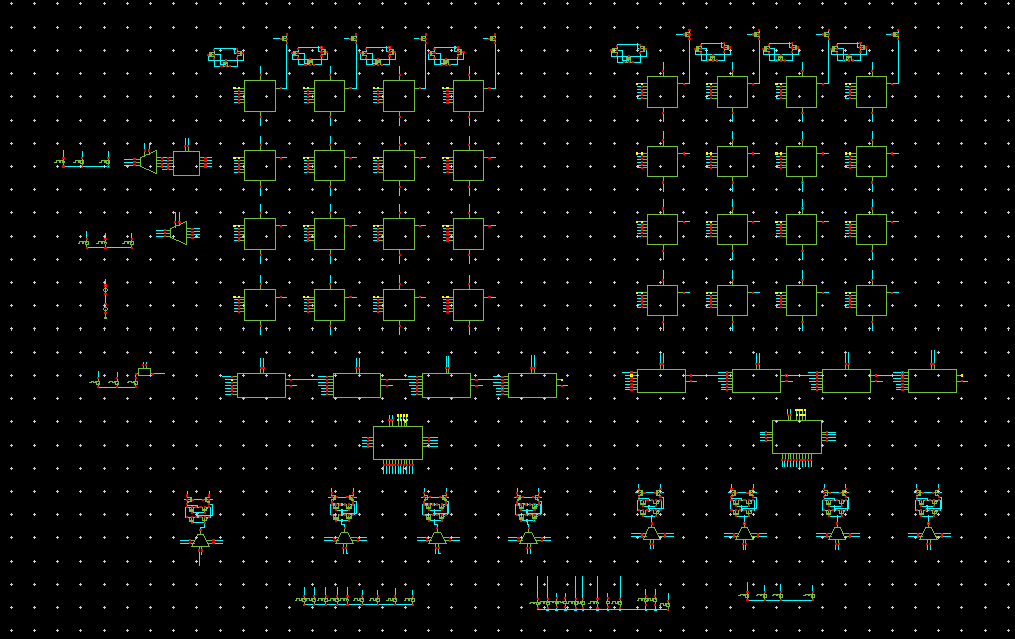
\includegraphics[width=1.0\textwidth]{full_design.png}
\caption{The Complete Integrated Design for In-Memory Computation}
\label{fig:Figure}
\end{figure}

\section{Overview}
\paragraph{}
After discussing each and every component of the design, the final integrated system looks something like as shown in Figure 6.1. It is a 8 word memory with each word corresponding to 4 bits. All the operations in any order can now be performed by giving the appropriate control pulses.

\section{Simulation Methodology}
\paragraph{}

In Cadence ADE it is possible to link a voltage source to a bit stream by just specifying the path of the bit stream and sampling period. This bit stream is generated from an Assembly Language code which can be easily written for the operations being performed. A python code working as an Assembler converts the Assembly code to these bit stream files. So when the execution is done in ADEL in Cadence, those files are taken as control signals to the circuit. 

This kind of methodology makes it easy to simulate and also perform basic tasks like some arithmetic, logical or both the operations on 4 bit words.

\begin{figure}[H]
\centering
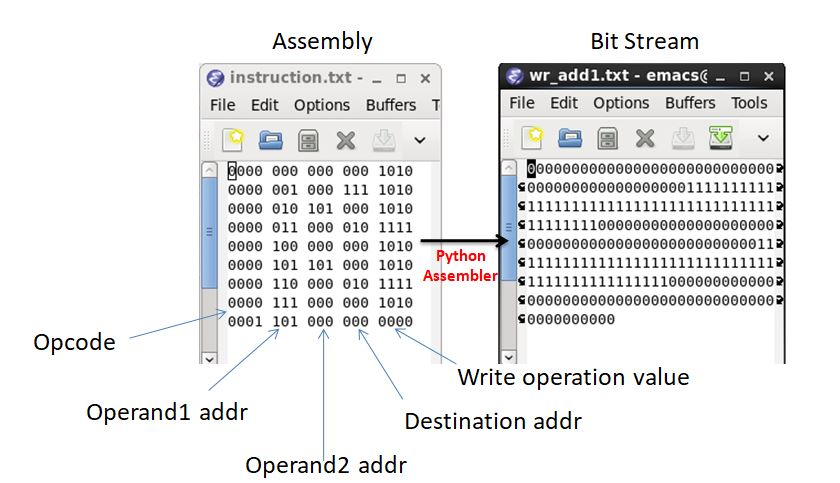
\includegraphics[width=1.0\textwidth]{simulation.JPG}
\caption{Conversion of Assembly Code to bit stream using Assembler}
\label{fig:Figure}
\end{figure}

The operands are read from the address specified in the code , result is computed and then is stored in stored back at a location specified by the code. The following is the format for the Assembly code : OPCODE; ADDRESS1; ADDRESS2; DESTINATION REGISTER; VALUE TO BE WRITTEN IN THE MEMORY( this value is only used when we have to write something in the memory directly. ) 

\begin{figure}[H]
\centering
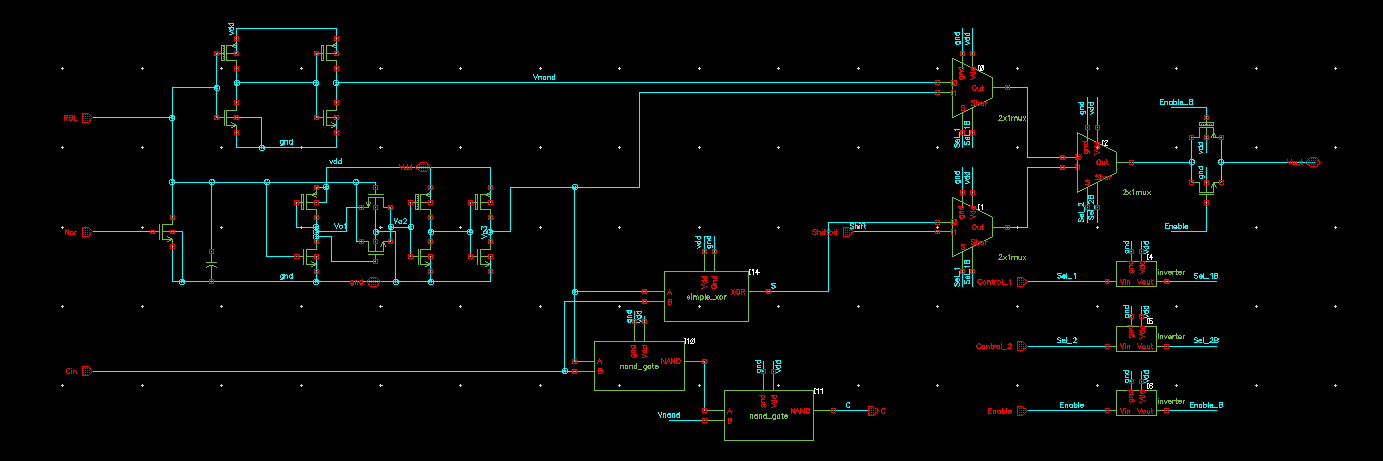
\includegraphics[width=1.0\textwidth]{complete_compute_unit.png}
\caption{The Compute Unit with Logical and Arithmetic operations}
\label{fig:Figure}
\end{figure}

\section{The Control Signals}
\paragraph{}

\begin{enumerate}
\item Write Controls(4x2 array):
\begin{enumerate}
\item There are 2($\log_2$ 4) row address signal that determines the row in which data is to be written. 
\item There are 2(For 2 block) precharge signals, which will only precharge the block where data is to be written, thus saving power.
\item There are 2 column enable signal, which will enable the write driver of the block where data is to be written, thus saving power. 
\item Each write driver is feed in by a 2x1 MUX which selects data to be written(0-Data input by user and 1-Data from compute block) 
\item The row address and column enable signals need to be given before starting the write operation as there is a certain finite delay. The final write\_en signal turns on the WWL thus starting the write operation.  
\end{enumerate}
\item Read  Controls:
\begin{enumerate}
\item There are 2($\log_2$ 4) row address signal that determines the row in which data is to be read from.In case of binary operation like NAND,NOR,XOR,ADD,the RBL is charged once the data is read from a single row, then Row address is changed and again data is read thus computing the appropriate output.  
\item There are 2(For 2 block) precharge signals, which will only precharge the block where data is to be read from, thus saving power.
\item The row address are given before starting of read operation as there is a finite delay. The final read\_en signal turns on the RWL thus starting the read operation.For binary operations this read\_en signal will turn on after certain interval to read the data from next row.  
\end{enumerate}
\item Compute  Controls:
\begin{enumerate}
\item There are 2(For 2 block) Block\_en signals, which will only enable operation of any 1 of the block from where Vout will come, as the Vout of all blocks are connected, it is very necessary that at any given time, at-most 1 block\_en is on.
\item There are 2 operation\_select signals which control a 4x1 MUX inside the compute unit. These signal decide what will be the value of Vout.{OP1,OP0} = {00-NOR,NAND,NOT},{01-XOR},{10-SUM},{11-Shift}.
\item Finally as seen in last signals NAND and NOR come from same port, so if NOR operation is needed , a separate Signal for it is given, that is NOR operation. 
\end{enumerate}
\item Shift Controls:
\begin{enumerate}
\item There are enable signals(en \& enb) to enable the shift operation. 
\item The S Signal is the direction of shift select signal, if S = 1 \& Sb = 0 , it is right shift and if S = 0 \& Sb = 1, it is right shift.
\item Signals enW and en1 are used to discharge and charge the write lines and read lines respectively, because before DRAM is read, the RBL of DRAM must be pre-charged(en1).
\item the out signal is used to pre-charge the RBL of DRAM for the final output of the shift. 
\item The readP and writeP signal pulses are necessary to activate the periodic write and read process of the DRAM in order to shift from one cell to the other. 
\end{enumerate}

\end{enumerate}

\begin{figure}[H]
\centering
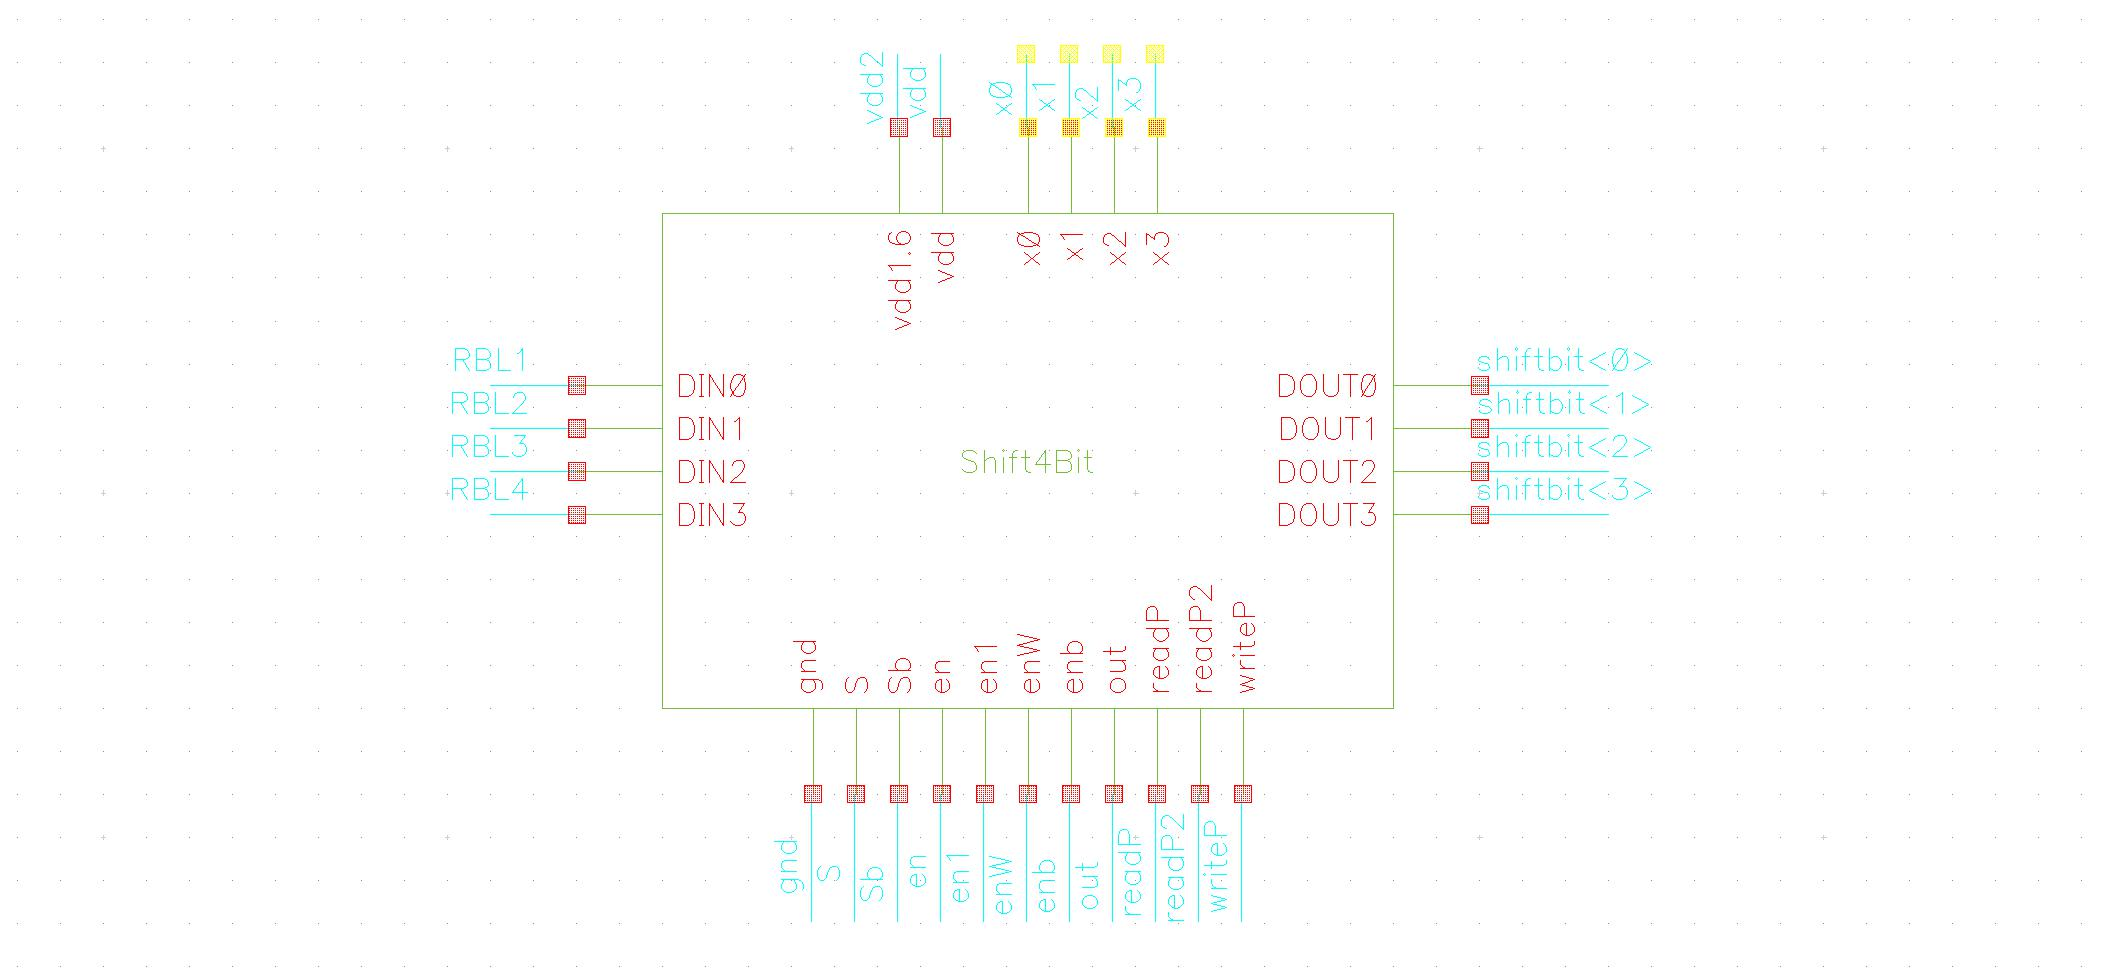
\includegraphics[width=1.2\textwidth]{shiftsym.jpg}
\caption{The shift block and it's control signals}
\label{fig:Figure}
\end{figure}